\documentclass[a4paper,12pt]{report}
\usepackage[left=30mm,right=30mm,top=30mm,bottom=30mm]{geometry}
\usepackage{booktabs}
\usepackage{amsmath}
\usepackage{setspace}
\usepackage{graphicx}
\usepackage[nodayofweek]{datetime}
\newdate{mydate}{9}{11}{2023}
\usepackage{appendix}
\usepackage{afterpage}
\usepackage{caption}
\usepackage{subcaption}
\usepackage{tikz}
\usetikzlibrary{arrows.meta}
\usepackage{cite}


\begin{document}
	\begin{titlepage}
		\begin{center}
			\begin{spacing}{1}
				\textit{\large Seminar Report \\}
				\vspace{5mm}
				\textbf{\Large Hall's Theorem}
				\vspace{1cm}
				\vspace{\fill}
			\end{spacing}
			\begin{spacing}{1}
				\textit{\large Report}\\
				\vspace{4mm}
				\textit{Submitted by\\}
				\vspace{4mm}
				\textbf{\large Himanshu Prajapati}\\
				\vspace{2mm}
				\textbf{Roll no. 222123026}\\
				\textbf{M.Sc. Mathematics and Computing}\\
				\vspace{2mm}
				\vspace{\fill}
			\end{spacing}
			
			\begin{figure}[h!]
				\centering
				\includegraphics[scale=0.15]{IITG_logo}
			\end{figure}
			\vspace{0.5cm}
			\begin{spacing}{1}
				\textbf{\Large Indian Institute of Technology \\}
				\vspace{4mm}
				\textbf{\large Guwahati-781039,India \\}
				\vspace{4mm}
			\end{spacing}
			\displaydate{mydate} 
		\end{center}
	\end{titlepage}
         
         	
         	\section*{Graph}
         	\subsection*{Definition}
         	A graph is an ordered triple $G = (V(G), E(G), I_G)$, where:- $V(G)$ is a nonempty set.- $E(G)$ is a set disjoint from $V(G)$.
         	- $I_G$ is an "incidence" relation that associates with each element of $E(G)$ an unordered pair of elements (same or distinct) of $V(G)$.
         	
         	Elements of $V(G)$ are called the vertices (or nodes or points) of $G$, and elements of $E(G)$ are called the edges (or lines) of $G$. $V(G)$ and $E(G)$ are the vertex set and edge set of $G$, respectively.
         	
         	If, for the edge $e$ of $G$, $I_G(e) = \{u, v\}$, we write $I_G(e) = uv$.
         	
         	\subsection*{Example:}
         	If $V(G) = \{v_1, v_2, v_3, v_4, v_5\}$, $E(G) = \{e_1, e_2, e_3, e_4, e_5, e_6\}$, and $I_G$ is given by:
         	- $I_G(e_1) = \{v_1, v_5\}$
         	- $I_G(e_2) = \{v_2, v_3\}$
         	- $I_G(e_3) = \{v_2, v_4\}$
         	- $I_G(e_4) = \{v_2, v_5\}$
         	- $I_G(e_5) = \{v_2, v_5\}$
         	- $I_G(e_6) = \{v_3, v_3\}$
         	
         	Then $(V(G), E(G), I_G)$ is a graph.
         	
         		\begin{figure}[h!]
         		\centering
         		
         		\includegraphics[scale=1]{Figure1}
         		\caption{Graph  $(V(G), E(G), I_G)$ described in Example}
         	\end{figure}
         
    	
    	\subsection*{Some Definitions Related to Graph}
    	\begin{enumerate}
    		\item A subset $M$ of the edge set $E$ of a loopless graph $G$ is called independent if no two edges of $M$ are adjacent in $G$.
    		
    		\item  A matching in $G$ is a set of independent edges.
    		 
    		\item An edge covering of $G$ is a subset $L$ of $E$ such that every vertex of $G$ is incident to some edge of $L$ .Hence, an edge covering of $G$ exists if and only if $\gamma > 0$.
    		
    		\item A matching $M$ of $G$ is maximum if $G$ has no matching $M_0$ with $|M_0| > |M|$. $M$ is maximal if $G$ has no matching $M_0$ strictly containing $M$. $|M^* (G)|$ is the cardinality of a maximum matching, and $|C^* (G)|$ is the size of a minimum edge covering of $G$.
    		
    		\item A set $S$ of vertices of $G$ is said to be saturated by a matching $M$ of $G$ or $M$-saturated if every vertex of $S$ is incident to some edge of $M$. A vertex $v$ of $G$ is $M$-saturated if $fv$ is $M$-saturated. $v$ is $M$-unsaturated if it is not $M$-saturated.
    	\end{enumerate}
    
    \section*{Bipartite Graph}
    \subsection*{Definition}
    A graph is bipartite if its vertex set can be partitioned into two nonempty subsets $X$ and $Y$ such that each edge of $G$ has one end in $X$ and the other in $Y$. The pair $(X, Y)$ is called a bipartition of the bipartite graph. The bipartite graph $G$ with bipartition $(X, Y)$ is denoted by $G[X, Y]$.
    \subsection*{Example:}
\begin{figure}[ht]
	\centering
	    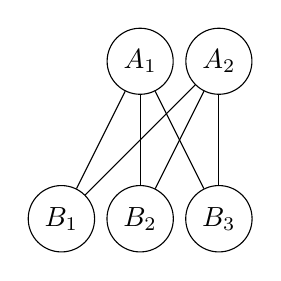
\begin{tikzpicture}
		% Set the vertices of the first part
		\foreach \x in {1,2}
		\node[draw, circle] (A\x) at (\x,0) {$A_\x$};
		
		% Set the vertices of the second part
		\foreach \y in {1,2,3}
		\node[draw, circle] (B\y) at (\y-1,-2) {$B_\y$};
		
		% Connect vertices with edges
		\foreach \x in {1,2}
		\foreach \y in {1,2,3}
		\draw (A\x) -- (B\y);
		
	\end{tikzpicture}
\caption{A bipartite graph $K_2,_3$}
\end{figure}
     	
    \section*{Matching in Bipartite Graph}
	
	\subsection*{Assignment Problem}
	Suppose in a factory there are \(n\) jobs \(j_1, j_2, \ldots, j_n\) and \(s\) workers \(w_1, w_2, \ldots, w_s\). Also, suppose that each job \(j_i\) can be performed by a certain number of workers, and each worker \(w_j\) has been trained to do a certain number of jobs. Is it possible to assign each of the \(n\) jobs to a worker who can do that job so that no two jobs are assigned to the same worker?
	
	We convert this job assignment problem into a problem in graphs as follows: Form a bipartite graph \(G\) with bipartition \(J, W\), where \(J = \{j_1, j_2, \ldots, j_n\}\) and \(W = \{w_1, w_2, \ldots, w_s\}\), and make \(j_i\) adjacent to \(w_j\) if and only if worker \(w_j\) can do the job \(j_i\). Then our assignment problem translates into the following graph problem: Is it possible to find a matching in \(G\) that saturates all the vertices of \(J\)?
	
	A solution to the above matching problem in bipartite graphs has been given by Hall.
	
	For a subset \(S \subseteq V\) in a graph \(G\), \(N(S)\) denotes the neighbor set of \(S\), that is, the set of all vertices, each of which is adjacent to at least one vertex in \(S\).

	
		
		\subsection*{Definition}
		Let $G$ be a bipartite graph on the parts $X$ and $Y$, and let $S$ be a matching of $G$. If every vertex in $X$ is covered by an edge of $S$, then we say that $S$ is a perfect matching of $X$ into $Y$.
		
		For a graph $G$ and a subset $T$ of $V(G)$, we let $N_G(T)$ denote the set of vertices of $G$ that are adjacent to some vertex in $T$, that is,
		\[
		N_G(T) := \{v \in V(G) \,|\, vw \in E(G) \text{ for some } w \in T\}.
		\]
		
		Observe that if $G$ is bipartite on the parts $A$ and $B$, then $N_G(T) \subseteq B$ for any $T \subseteq A$.
		
		\section*{Hall's Theorem}
		\textit{For a bipartite graph $G$ on the parts $X$ and $Y$, the following conditions are equivalent.
			\begin{enumerate}
				\item[(a)] There is a perfect matching of $X$ into $Y$.
				\item[(b)] For each $T \subseteq X$, the inequality $|T| \leq |N_G(T)|$ holds.
		\end{enumerate}}
		
		\subsection*{Proof:}
		\begin{enumerate}
		    	\item[(a) $\Rightarrow$ (b):] Let $S$ be a perfect matching of $X$ into $Y$. As $S$ is a perfect matching, for every $x \in X$, there exists a unique $y_x \in Y$ such that $xy_x \in S$. Define the map $f : X \to Y$ by $f(x) = y_x$. Since $S$ is a matching, the function $f$ is injective. Therefore, for any $T \subseteq X$, we see that $|T| = |f(T)| \leq |N_G(T)|$ because $f(T) \subseteq N_G(T)$.
			
			\item[(b) $\Rightarrow$ (a):] Conversely, suppose that $|T| \leq |N_G(T)|$ for each $T \subseteq X$. We will prove that there exists a perfect matching of $X$ into $Y$ by induction on $n := |X|$. If $n = 1$, then the only vertex $x$ in $X$ must be adjacent to some vertex $y$ in $Y$ by condition (b), and, therefore, $\{xy\}$ is a perfect matching of $X$ into $Y$. Now assume that every bipartite graph on the parts $X_0$ and $Y_0$ with $|X_0| < |X|$ and satisfying condition (b) has a perfect matching of $X_0$ into $Y_0$. We split the rest of the proof into two cases.
			
			\textbf{Case 1:} For every nonempty proper subset $T$ of $X$ (that is, $T \subset X$), the strict inequality $|T| < |N_G(T)|$ holds. Take $x \in X$ and $y \in $NG($\{x\}$). Let $G_0$ be the bipartite graph we obtain by removing $x$ and $y$ (and the edges incident to them) from $G$. Now for every subset $A$ of $X \setminus \{x\}$, we see that
			\[
			|N_{G_0}(A)| \geq |N_G(A)| - 1 \geq |A|,
			\]
			where the last inequality holds because $A$ is a strict subset of $X$. By induction hypothesis, there exists a perfect matching $S_0$ in $G_0$ of $X \setminus \{x\}$ into $Y \setminus \{y\}$. It is clear now that $S_0 \cup \{xy\}$ is a perfect matching in $G$ of $X$ into $Y$.
			
			\textbf{Case 2:} There exists a nonempty proper subset $A$ of $X$ such that $|A| = |N_G(A)|$. Let $G_1$ be the subgraph of $G$ induced by the set of vertices $A \cup N_G(A)$, and let $G_2$ be the subgraph of $G$ we obtain by removing $A \cup N_G(A)$ (and their incident edges) from $G$. It is clear that $G_1 = (A, N_G(A))$ and $G_2 = (X \setminus A, Y \setminus N_G(A))$ are bipartite graphs.
			
			Let us show that both $G_1$ and $G_2$ satisfy condition (b). To show that $G_1$ satisfies (b), take $T \subseteq A$. It follows by the way $G_1$ was constructed that $N_{G_1}(T) = N_G(T)$. As a result, $|N_{G_1}(T)| = |N_G(T)| \geq |T|$. Then $G_1$ satisfies condition (b). In order to argue that $G_2$ also satisfies condition (b), take $T_0 \subseteq X \setminus A$ and observe that $N_{G_2}(T_0 \cup A) = N_G(A) \cup N_{G_2}(T_0)$, where the union on the right-hand side is disjoint. Since $|N_{G_2}(T_0 \cup A)| \geq |T_0 \cup A|$ and $|N_G(A)| = |A|$, $|N_{G_2}(T_0)| = |N_{G_2}(T_0 \cup A)| - |N_{G_1}(A)| \geq |T_0 \cup A| - |A| = (|T_0| + |A|) - |A| = |T_0|$. Therefore, $G_2$ also satisfies condition (b).
			
			Since $|A| < |X|$ and $|X \setminus A| < |X|$, our induction hypothesis guarantees the existence of a perfect matching $S_1$ in $G_1$ of $A$ into $N_G(A)$ and a perfect matching $S_2$ in $G_2$ of $X \setminus A$ into $Y \setminus N_G(A)$. Then it follows from the construction of $G_1$ and $G_2$ that $S_1 \cup S_2$ is a perfect matching in $G$ of $X$ into $Y$, which concludes the proof.
		\end{enumerate}
	 
	 \begin{figure}[ht]
	 	\centering
	 	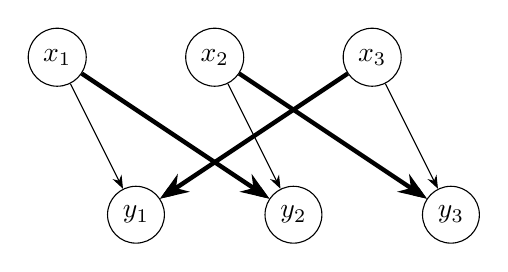
\begin{tikzpicture}
	 		% Vertices in set X
	 		\node[draw, circle] (x1) at (0, 0) {$x_1$};
	 		\node[draw, circle] (x2) at (2, 0) {$x_2$};
	 		\node[draw, circle] (x3) at (4, 0) {$x_3$};
	 		% Vertices in set Y
	 		\node[draw, circle] (y1) at (1, -2) {$y_1$};
	 		\node[draw, circle] (y2) at (3, -2) {$y_2$};
	 		\node[draw, circle] (y3) at (5, -2) {$y_3$};
	 		% Edges
	 		\draw[-{Stealth}] (x1) -- (y1);
	 		\draw[-{Stealth}] (x1) -- (y2);
	 		\draw[-{Stealth}] (x2) -- (y2);
	 		\draw[-{Stealth}] (x2) -- (y3);
	 		\draw[-{Stealth}] (x3) -- (y1);
	 		\draw[-{Stealth}] (x3) -- (y3);
	 		% Boldfaced matching edges
	 		\draw[-{Stealth}, ultra thick] (x1) -- (y2);
	 		\draw[-{Stealth}, ultra thick] (x2) -- (y3);
	 		\draw[-{Stealth}, ultra thick] (x3) -- (y1);
	 	\end{tikzpicture}
	 	\caption{Illustration of a matching with boldfaced edges.}
	 \end{figure}
	
	\vspace{1cm}
	  \textbf{ We now give some important consequences of Hall’s theorem;}
	    \hfill
		\subsection*{Theorem}
		
		\textit{A $k(>1)$-regular bipartite graph is 1-factorable}
		
		\subsection*{Proof:}
		Let $G$ be a $k$-regular bipartite graph with bipartition $X$ and $Y$. Then, $E(G)$ is the set of edges incident to the vertices of $X$ and is also equal to the set of edges incident to the vertices of $Y$. Hence, $k|X| = |E(G)| = k|Y|$, and therefore $|X| = |Y|$. 
		
		Now, consider any subset $S \subseteq X$. By the definition of a bipartite graph, the neighborhood of $S$, denoted as $N(S)$, is contained in $Y$, and $N(N(S))$ contains $S$. 
		
		Let $E_1$ and $E_2$ be the sets of edges of $G$ incident to $S$ and $N(S)$, respectively. Then, $E_1 \cup E_2$ contains all the edges of $G$ incident to vertices in $S$. We have $|E_1| = k|S|$ and $|E_2| = k|N(S)|$. Therefore, since $|E_1| + |E_2| = |E_1 \cup E_2| \leq k|S|$, it follows that $k|N(S)| \leq k|S|$. 
		
		As $k > 1$, we can conclude that $|N(S)| \leq |S|$. So, by Hall's theorem (Theorem 5.5.2), $G$ has a matching that saturates all the vertices of $X$, which means that $G$ has a perfect matching $M$. 
		
		Deletion of the edges in $M$ from $G$ results in a $(k - 1)$-regular bipartite graph. 
		
		Repeated application of this argument shows that $G$ is 1-factorable.
	
	\begin{center}
		\rule{\textwidth}{1.5pt}
	\end{center}

  % Specify the bibliography style
 %\cite{example , another}
  \bibliographystyle{plain}
  \bibliography{refrence}
   


\end{document}
